\documentclass{beamer}
\usepackage[utf8]{inputenc}

\usetheme{Madrid}
\usecolortheme{default}
\usepackage{amsmath,amssymb,amsfonts,amsthm}
\usepackage{mathtools}
\usepackage{txfonts}
\usepackage{tkz-euclide}
\usepackage{listings}
\usepackage{adjustbox}
\usepackage{tfrupee}
\usepackage{array}
\usepackage{gensymb}
\usepackage{tabularx}
\usepackage{gvv}
\usepackage{lmodern}
\usepackage{circuitikz}
\usepackage{tikz}
\lstset{literate={·}{{$\cdot$}}1 {λ}{{$\lambda$}}1 {→}{{$\to$}}1}
\usepackage{graphicx}

\setbeamertemplate{page number in head/foot}[totalframenumber]

\usepackage{tcolorbox}
\tcbuselibrary{minted,breakable,xparse,skins}

\definecolor{bg}{gray}{0.95}
\DeclareTCBListing{mintedbox}{O{}m!O{}}{%
  breakable=true,
  listing engine=minted,
  listing only,
  minted language=#2,
  minted style=default,
  minted options={%
    linenos,
    gobble=0,
    breaklines=true,
    breakafter=,,
    fontsize=\small,
    numbersep=8pt,
    #1},
  boxsep=0pt,
  left skip=0pt,
  right skip=0pt,
  left=25pt,
  right=0pt,
  top=3pt,
  bottom=3pt,
  arc=5pt,
  leftrule=0pt,
  rightrule=0pt,
  bottomrule=2pt,
  toprule=2pt,
  colback=bg,
  colframe=orange!70,
  enhanced,
  overlay={%
    \begin{tcbclipinterior}
    \fill[orange!20!white] (frame.south west) rectangle ([xshift=20pt]frame.north west);
    \end{tcbclipinterior}},
  #3,
}
\lstset{
    language=C,
    basicstyle=\ttfamily\small,
    keywordstyle=\color{blue},
    stringstyle=\color{orange},
    commentstyle=\color{green!60!black},
    numbers=left,
    numberstyle=\tiny\color{gray},
    breaklines=true,
    showstringspaces=false,
}

\title{7.4.20}
\date{September 20, 2025}
\author{Bhargav - EE25BTECH11013}

\begin{document}

\frame{\titlepage}

\begin{frame}{Question}
The point diametrically opposite to the point $P \brak{1 , 0}$ on the circle 
\begin{align}
x^2 +y^2 + 2x + 2y - 3 =  0
\end{align} 
is
\end{frame}

\begin{frame}{Solution}
Let the diametrically opposite point be $\vec{Q}$.\\
The equation of the circle is:($\vec{V}$ is an identity matrix of order = 2)
\begin{align}
\vec{x^T}\vec{V}\vec{x} + 2\vec{u^T}\vec{x} + f = 0 
\end{align}

\begin{align}
\vec{u} = \myvec{u \\ v} = \myvec{1 \\ 1}
\end{align}

The center of the circle $\vec{c}$ is
\begin{align}
\implies \vec{c} = -\vec{u} = \myvec{-1 \\ -1}
\end{align}
\end{frame}

\begin{frame}{Solution}
Using the property of diametrically opposite points:
\begin{align}
\vec{c} = \frac{\vec{P}+\vec{Q}}{2}
\end{align}

\begin{align}
\vec{Q} = 2\vec{c} - \vec{P} = 2\myvec{-1 \\ -1} - \myvec{1 \\ 0} = \myvec{-3 \\ -2}
\end{align}
\end{frame}

\begin{frame}{Plot}
\begin{figure}[h!]
    \centering
    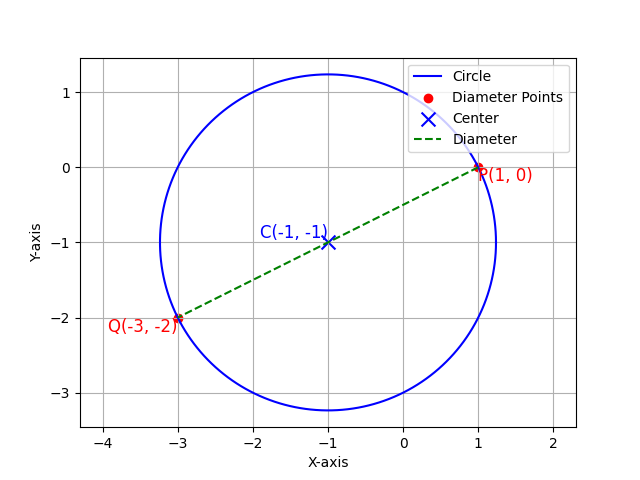
\includegraphics[height=0.5\textheight, keepaspectratio]{figs/Figure_1.png}
    \label{figure_1}
\end{figure}
\end{frame}

\begin{frame}[fragile]
    \frametitle{C Code}
    \begin{lstlisting}
#include <stdio.h>
#include <math.h>

int xcenter(int c, int p, int m, int n){
    return (m*c + n*p)/(m+n);
}

int ycenter(int c, int p, int m, int n){
    return (m*c + n*p)/(m+n);
}
double dist(int x1, int y1, int x2, int y2){
    return sqrt((x1-x2)*(x1-x2) + (y1-y2)*(y1-y2));
}


    \end{lstlisting}
\end{frame}
\begin{frame}[fragile]
    \frametitle{Python + C Code}
    \begin{lstlisting}
import ctypes
import numpy as np 
import matplotlib.pyplot as plt

lib = ctypes.CDLL("./libcode.so")

lib.xcenter.argtypes = [ctypes.c_int, ctypes.c_int, ctypes.c_int, ctypes.c_int]
lib.xcenter.restype = ctypes.c_int

lib.ycenter.argtypes = [ctypes.c_int, ctypes.c_int, ctypes.c_int, ctypes.c_int]
lib.ycenter.restype = ctypes.c_int

lib.dist.argtypes = [ctypes.c_int, ctypes.c_int, ctypes.c_int, ctypes.c_int]
lib.dist.restype = ctypes.c_double

c = np.array([-1, -1])




    \end{lstlisting}
\end{frame}
\begin{frame}[fragile]
    \frametitle{Python + C Code}
    \begin{lstlisting}

p = np.array([1, 0])


x = lib.xcenter(c[0], p[0], 2, -1)
y = lib.ycenter(c[1], p[1], 2, -1)
q = np.array([x, y])
print("The point Q is ", q)

r = lib.dist(c[0], c[1], p[0], p[1])

theta = np.linspace(0, 2*np.pi, 200)
circle_x = c[0] + r*np.cos(theta)
circle_y = c[1] + r*np.sin(theta)

fig, ax = plt.subplots()

ax.plot(circle_x, circle_y, color="blue", label="Circle")
ax.scatter([p[0], q[0]], [p[1], q[1]], color="red", label="Diameter Points")


    \end{lstlisting}
\end{frame}
\begin{frame}[fragile]
    \frametitle{Python + C Code}
    \begin{lstlisting}
ax.scatter(c[0], c[1], color="blue", marker="x", s=100, label="Center")
ax.plot([p[0], q[0]], [p[1], q[1]], "g--", label="Diameter")
ax.set_aspect("equal", adjustable="datalim")
ax.set_xlabel("X-axis")
ax.set_ylabel("Y-axis")
ax.text(c[0], c[1], f"C({int(c[0])}, {int(c[1])})", fontsize=12, color="blue", ha="right", va="bottom")
ax.text(p[0], p[1], f"P({int(p[0])}, {int(p[1])})", fontsize=12, color="red", ha="left", va="top")
ax.text(q[0], q[1], f"Q({int(q[0])}, {int(q[1])})", fontsize=12, color="red", ha="right", va="top")
ax.legend()
ax.legend(loc="upper right")
ax.grid(True)
plt.savefig("/Users/bhargavkrish/Desktop/BackupMatrix/ee25btech11013/matgeo/7.4.20/figs/Figure_1.png")
plt.show()


    \end{lstlisting}
\end{frame}

\begin{frame}[fragile]
    \frametitle{Python Code}
    \begin{lstlisting}
import numpy as np
import matplotlib.pyplot as plt
c = np.array([-1, -1])
p = np.array([1, 0])
def diam_opposite(center, point):
    return 2*center - point
def distance(pt1, pt2):
    return np.sqrt((pt1[0]-pt2[0])**2 + (pt1[1]-pt2[1])**2)
q = diam_opposite(c, p)
r = distance(c, p)
print("The point Q is:", q)
print("Radius r:", r)

theta = np.linspace(0, 2*np.pi, 200)
circle_x = c[0] + r*np.cos(theta)
circle_y = c[1] + r*np.sin(theta)
fig, ax = plt.subplots()
    \end{lstlisting}
\end{frame}
\begin{frame}[fragile]
    \frametitle{Python Code}
    \begin{lstlisting}
ax.plot(circle_x, circle_y, color="blue", label="Circle")
ax.scatter([p[0], q[0]], [p[1], q[1]], color="red", label="Diameter Points")
ax.scatter(c[0], c[1], color="blue", marker="x", s=100, label="Center")
ax.plot([p[0], q[0]], [p[1], q[1]], "g--", label="Diameter")
ax.text(c[0], c[1], f"C({c[0]}, {c[1]})", fontsize=12, color="blue", ha="right", va="bottom")
ax.text(p[0], p[1], f"P({p[0]}, {p[1]})", fontsize=12, color="red", ha="left", va="top")
ax.text(q[0], q[1], f"Q({q[0]}, {q[1]})", fontsize=12, color="red", ha="right", va="top")
ax.set_aspect("equal", adjustable="datalim")
ax.set_xlabel("X-axis")
ax.set_ylabel("Y-axis")
ax.legend(loc="upper right")
ax.grid(True)
plt.savefig("/Users/bhargavkrish/Desktop/BackupMatrix/ee25btech11013/matgeo/7.4.20/figs/Figure_1.png")  
plt.show()

    \end{lstlisting}
\end{frame}


\end{document}

